\documentclass[11pt]{article}
\usepackage[margin=0.9in]{geometry}
\usepackage[T1]{fontenc}
\usepackage[utf8]{inputenc}
\usepackage{hyperref}
\usepackage{xcolor}
\usepackage{tikz}
\usetikzlibrary{arrows.meta,positioning,fit,backgrounds,shapes.geometric}
\usepackage{amsmath}
\usepackage{listings}
\usepackage{booktabs}
\usepackage{longtable}
\usepackage{enumitem}

\hypersetup{colorlinks=true,linkcolor=blue,urlcolor=blue}

\lstdefinestyle{code}{
  basicstyle=\ttfamily\footnotesize,
  breaklines=true,
  frame=single,
  columns=fullflexible,
  keepspaces=true,
  showstringspaces=false
}

\title{Llama Inference C++: Full Forward Pass Handbook\\\large Entry Point to Token Generation (with Color Diagrams)}
\author{llama\_inference\_cpp}
\date{\today}

\begin{document}
\maketitle
\tableofcontents
\newpage

\section{Purpose}
This handbook explains the full runtime path in the current C++ codebase:
\begin{itemize}[leftmargin=*]
  \item from CLI entry point,
  \item through model loading and forward-pass blocks,
  \item to sampling and final token output.
\end{itemize}
It is structured block-by-block, with diagrams and file/function mapping.

\section{Code map (where each step lives)}
\begin{longtable}{p{0.30\linewidth} p{0.62\linewidth}}
\toprule
\textbf{File} & \textbf{Responsibility} \\
\midrule
\endhead
\texttt{src/main.cpp} & CLI entry point, argument parsing, invokes model/tokenizer load and generation. \\
\texttt{src/engine\_lifecycle.cpp} & Constructor/destructor, checkpoint mmap, weight pointer mapping, run-state allocation. \\
\texttt{src/tokenizer.cpp} & Tokenizer binary loading, encode (BPE), decode piece-by-piece. \\
\texttt{src/engine\_math\_kernels.cpp} & Primitive compute blocks: RMSNorm, softmax, matmul (GEMV style). \\
\texttt{src/engine\_forward.cpp} & Full transformer forward pass for one token at one position. \\
\texttt{src/engine\_sampling.cpp} & Sampling methods (argmax, multinomial, top-p) and autoregressive generation loop. \\
\texttt{include/llama\_engine.hpp} & Public class/struct declarations and private engine internals. \\
\bottomrule
\end{longtable}

\section{Color Legend}
\begin{itemize}[leftmargin=*]
  \item \textcolor{blue!70!black}{Blue}: I/O boundaries (token input, output text)
  \item \textcolor{green!50!black}{Green}: normalization and stabilizing operations
  \item \textcolor{orange!85!black}{Orange}: linear projections/matmul blocks
  \item \textcolor{purple!70!black}{Purple}: attention-specific operations
  \item \textcolor{red!70!black}{Red}: nonlinear or sampling decisions
\end{itemize}

\section{Diagram 1: End-to-end runtime path}
\begin{center}
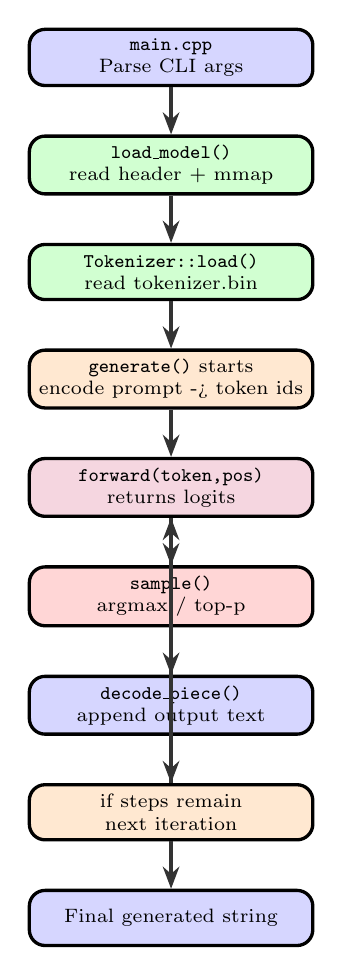
\begin{tikzpicture}[
  node distance=6mm and 7mm,
  >={Stealth[length=2.8mm]},
  every node/.style={font=\scriptsize, align=center},
  io/.style={draw, rounded corners=2mm, very thick, fill=blue!16, minimum width=36mm, minimum height=7mm},
  load/.style={draw, rounded corners=2mm, very thick, fill=green!18, minimum width=36mm, minimum height=7mm},
  proc/.style={draw, rounded corners=2mm, very thick, fill=orange!18, minimum width=36mm, minimum height=7mm},
  fwd/.style={draw, rounded corners=2mm, very thick, fill=purple!16, minimum width=36mm, minimum height=7mm},
  samp/.style={draw, rounded corners=2mm, very thick, fill=red!16, minimum width=36mm, minimum height=7mm},
  arrow/.style={->, very thick, color=black!80}
]

\node[io] (main) {\texttt{main.cpp}\\Parse CLI args};
\node[load, below=of main] (lm) {\texttt{load\_model()}\\read header + mmap};
\node[load, below=of lm] (ltok) {\texttt{Tokenizer::load()}\\read tokenizer.bin};
\node[proc, below=of ltok] (gen) {\texttt{generate()} starts\\encode prompt -> token ids};
\node[fwd, below=of gen] (fwd) {\texttt{forward(token,pos)}\\returns logits};
\node[samp, below=of fwd] (samp) {\texttt{sample()}\\argmax / top-p};
\node[io, below=of samp] (dec) {\texttt{decode\_piece()}\\append output text};
\node[proc, below=of dec] (loop) {if steps remain\\next iteration};
\node[io, below=of loop] (done) {Final generated string};

\draw[arrow] (main)--(lm);
\draw[arrow] (lm)--(ltok);
\draw[arrow] (ltok)--(gen);
\draw[arrow] (gen)--(fwd);
\draw[arrow] (fwd)--(samp);
\draw[arrow] (samp)--(dec);
\draw[arrow] (dec)--(loop);
\draw[arrow] (loop)--(fwd);
\draw[arrow] (loop)--(done);

\end{tikzpicture}
\end{center}

\section{Entry point block-by-block}
\subsection{1) CLI parsing in \texttt{main.cpp}}
The executable reads:
\begin{itemize}[leftmargin=*]
  \item checkpoint path,
  \item tokenizer path,
  \item prompt,
  \item generation controls: \texttt{steps}, \texttt{temperature}, \texttt{topp}, \texttt{seed}.
\end{itemize}
Then:
\begin{lstlisting}[style=code]
LlamaEngine engine;
engine.load_model(checkpoint);
Tokenizer tokenizer;
tokenizer.load(tokenizer_path, engine.config().vocab_size);
std::string text = engine.generate(tokenizer, prompt, steps, temperature, topp, seed);
\end{lstlisting}

\subsection{2) Model load path in \texttt{engine\_lifecycle.cpp}}
\begin{enumerate}[leftmargin=*]
  \item open checkpoint file,
  \item read \texttt{Config},
  \item map file into memory (
\texttt{mmap}),
  \item compute weight pointer offsets (
\texttt{memory\_map\_weights}),
  \item allocate run-state tensors and KV caches.
\end{enumerate}

\subsection{3) Tokenizer load/encode/decode in \texttt{tokenizer.cpp}}
\begin{itemize}[leftmargin=*]
  \item \texttt{load()}: reads token strings and scores from tokenizer binary.
  \item \texttt{encode()}: BOS prefix, UTF-8 byte handling, byte fallback, iterative BPE merges.
  \item \texttt{decode\_piece()}: token-id to printable piece conversion.
\end{itemize}

\section{Diagram 2: Forward pass compute graph (single decode step)}
\begin{center}
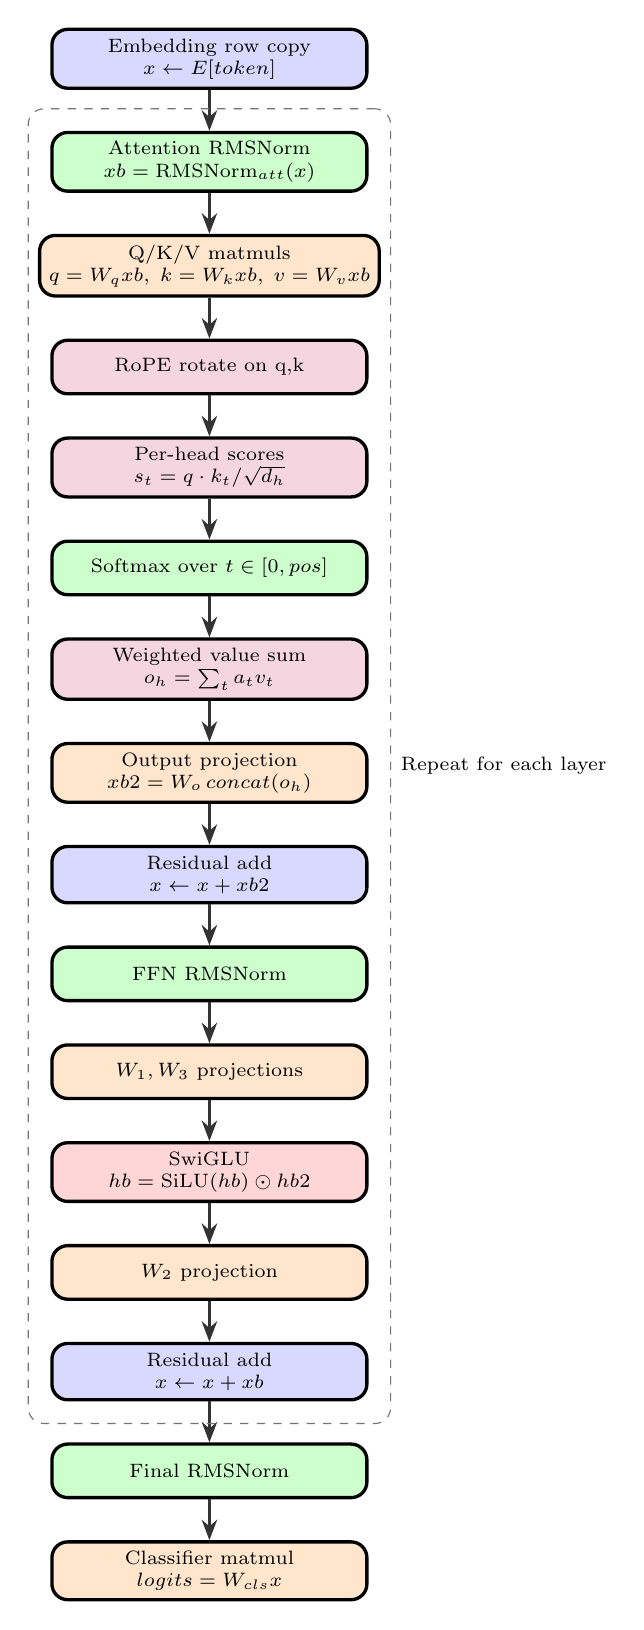
\begin{tikzpicture}[
  node distance=5.2mm and 6.2mm,
  >={Stealth[length=2.6mm]},
  every node/.style={font=\scriptsize, align=center},
  inout/.style={draw, rounded corners=2mm, very thick, fill=blue!15, minimum width=40mm, minimum height=6.8mm},
  norm/.style={draw, rounded corners=2mm, very thick, fill=green!20, minimum width=40mm, minimum height=6.8mm},
  lin/.style={draw, rounded corners=2mm, very thick, fill=orange!20, minimum width=40mm, minimum height=6.8mm},
  attn/.style={draw, rounded corners=2mm, very thick, fill=purple!16, minimum width=40mm, minimum height=6.8mm},
  nlin/.style={draw, rounded corners=2mm, very thick, fill=red!16, minimum width=40mm, minimum height=6.8mm},
  arrow/.style={->, very thick, color=black!80}
]

\node[inout] (embed) {Embedding row copy\\$x \leftarrow E[token]$};
\node[norm, below=of embed] (anorm) {Attention RMSNorm\\$xb = \mathrm{RMSNorm}_{att}(x)$};
\node[lin, below=of anorm] (qkv) {Q/K/V matmuls\\$q=W_qxb,\;k=W_kxb,\;v=W_vxb$};
\node[attn, below=of qkv] (rope) {RoPE rotate on q,k};
\node[attn, below=of rope] (score) {Per-head scores\\$s_t=q\cdot k_t/\sqrt{d_h}$};
\node[norm, below=of score] (soft) {Softmax over $t\in[0,pos]$};
\node[attn, below=of soft] (wsum) {Weighted value sum\\$o_h=\sum_t a_t v_t$};
\node[lin, below=of wsum] (wo) {Output projection\\$xb2=W_o\,concat(o_h)$};
\node[inout, below=of wo] (res1) {Residual add\\$x\leftarrow x+xb2$};
\node[norm, below=of res1] (fnorm) {FFN RMSNorm};
\node[lin, below=of fnorm] (w13) {$W_1, W_3$ projections};
\node[nlin, below=of w13] (swiglu) {SwiGLU\\$hb=\mathrm{SiLU}(hb)\odot hb2$};
\node[lin, below=of swiglu] (w2) {$W_2$ projection};
\node[inout, below=of w2] (res2) {Residual add\\$x\leftarrow x+xb$};
\node[norm, below=of res2] (finaln) {Final RMSNorm};
\node[lin, below=of finaln] (cls) {Classifier matmul\\$logits=W_{cls}x$};

\draw[arrow] (embed)--(anorm);
\draw[arrow] (anorm)--(qkv);
\draw[arrow] (qkv)--(rope);
\draw[arrow] (rope)--(score);
\draw[arrow] (score)--(soft);
\draw[arrow] (soft)--(wsum);
\draw[arrow] (wsum)--(wo);
\draw[arrow] (wo)--(res1);
\draw[arrow] (res1)--(fnorm);
\draw[arrow] (fnorm)--(w13);
\draw[arrow] (w13)--(swiglu);
\draw[arrow] (swiglu)--(w2);
\draw[arrow] (w2)--(res2);
\draw[arrow] (res2)--(finaln);
\draw[arrow] (finaln)--(cls);

\node[draw=black!55, dashed, rounded corners=2mm, fit=(anorm)(res2), inner sep=2.8mm, label={[black]right:Repeat for each layer}] {};
\end{tikzpicture}
\end{center}

\section{Forward pass block explanations in code order}
\subsection{A) Preparation}
In \texttt{engine\_forward.cpp}, the function caches local dimensions:
\texttt{dim, kv\_dim, kv\_mul, hidden\_dim, head\_size}.

\subsection{B) Embedding boundary}
It copies a single embedding row into \texttt{x}. This is the starting representation for current token position.

\subsection{C) Attention block per layer}
\begin{enumerate}[leftmargin=*]
  \item attention RMSNorm,
  \item Q/K/V matmuls,
  \item RoPE rotation for q/k channel pairs,
  \item score computation over cached timesteps,
  \item softmax to attention probabilities,
  \item weighted sum over value cache,
  \item output projection and residual add.
\end{enumerate}

\subsection{D) FFN block per layer}
\begin{enumerate}[leftmargin=*]
  \item FFN RMSNorm,
  \item \(W_1\) and \(W_3\) projections,
  \item SwiGLU gating,
  \item \(W_2\) projection,
  \item residual add.
\end{enumerate}

\subsection{E) Final logits}
After all layers:
\begin{itemize}[leftmargin=*]
  \item final RMSNorm,
  \item classifier matmul to produce logits for next token.
\end{itemize}

\section{Sampling and generation path}
In \texttt{engine\_sampling.cpp}:
\begin{itemize}[leftmargin=*]
  \item If \texttt{temperature==0}, choose argmax (deterministic).
  \item Else scale logits by temperature, softmax, then sample:
  \begin{itemize}
    \item full multinomial if top-p disabled,
    \item nucleus (top-p) truncation + sample otherwise.
  \end{itemize}
  \item Decode selected token piece and append to output text.
\end{itemize}

\section{Function reference (quick lookup)}
\begin{longtable}{p{0.3\linewidth} p{0.62\linewidth}}
\toprule
\textbf{Function} & \textbf{Purpose} \\
\midrule
\endhead
\texttt{load\_model()} & Reads config, mmaps checkpoint, maps weight pointers, allocates run state. \\
\texttt{Tokenizer::load()} & Loads tokenizer vocabulary and scores. \\
\texttt{Tokenizer::encode()} & Prompt text to token ids. \\
\texttt{forward(token,pos)} & One full transformer step returning logits. \\
\texttt{sample(...)} & Chooses next token id from logits distribution. \\
\texttt{generate(...)} & Full autoregressive loop from prompt to final text. \\
\bottomrule
\end{longtable}

\section{Practical reading order}
Recommended order if studying implementation deeply:
\begin{enumerate}[leftmargin=*]
  \item \texttt{src/main.cpp}
  \item \texttt{src/engine\_lifecycle.cpp}
  \item \texttt{src/tokenizer.cpp}
  \item \texttt{src/engine\_forward.cpp}
  \item \texttt{src/engine\_sampling.cpp}
  \item \texttt{src/engine\_math\_kernels.cpp}
\end{enumerate}

\end{document}
